\begin{figure}
\centering
\caption{How frequently participants measured the impact of their changes when using \unsafe to improve performance}
\label{fig:rq2:profiling}
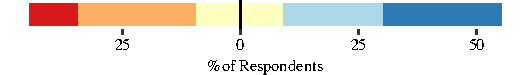
\includegraphics[width=\columnwidth]{figures/compiled/rq2_profiling.pdf}
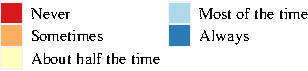
\includegraphics{figures/compiled/legends/legend_frequency_wrapped.pdf}
\end{figure}

Participants used \unsafe code because they perceived that it was more performant or ergonomic than safe alternatives, or that there were no safe alternatives at all.

\subsubsection{Unsafe Performs Better}
Some interview participants and \ArrayItemRounded{rq2.motivation.i.could.use.a.safe.pattern.but.unsafe.is.faster.or.more.space-efficient.}\% of survey respondents indicated that they would use \unsafe code when they perceived that it was faster or more space-efficient than an equivalent safe API. In these situations, participants usually identified a safe alternative, but they felt that it would be too expensive to use; \ilquote{so you could do it, right? But that would be some performance overhead}{12}. 

Most interview participants who attempted to use \unsafe to improve performance had implemented small-scale optimizations in existing applications. These typically involved eliminating runtime checks, which were seen as unnecessary due to local or global invariants. For example, one participant used an \unsafe API to consume a pointer to a string without checking if it contained valid UTF-8 characters. This pointer was provided by a foreign call to Python, which the participant reasoned would only ever provide text in a valid format. Another participant chose to store a heap allocation as a raw pointer in a static mutable variable instead of using one of Rust's safe static encapsulations, since they felt confident that the allocation would be valid for the duration of the program.


However, a few interview participants used \unsafe code to create entire components that were purpose-built to achieve performance.  In each situation, performance was seen as a functional requirement for the application domain: \ilquote{I write a serialization framework...And obviously a goal for it is to be extremely performant}{3}. A participant who took this approach found that it significantly increased the amount of \unsafe code in their application, but they felt that this was a reasonable compromise to achieve greater performance.

The \ArrayItemRounded{rq2.motivation.i.could.use.a.safe.pattern.but.unsafe.is.faster.or.more.space-efficient.}\% of survey respondents who reported using \unsafe code to improve performance did not have a strong tendency toward either large-scale or small-scale use. We found that \ArrayItemRounded{rq2.perf.scale.small-scale.optimizations}\% only pursued ``small-scale-optimizations in existing applications,'' \ArrayItemRounded{rq2.perf.scale.large-scale.components.purpose-built.for.performance.}\% only built new, ``large-scale components,'' and \ArrayItemRounded{rq2.perf.scale.both}\% used \unsafe code for performance in either situation.

\FPeval{\profilingmore}{round(\ArrayItem{rq2.profiling.about.half.the.time} + \ArrayItem{rq2.profiling.always} + \ArrayItem{rq2.profiling.most.of.the.time}, 0)}

Participants did not consistently measure the performance impact of \unsafe code. In some situations, they relied on their intuition to determine which design decisions would be best: \ilquote{I'll totally admit that...I think this is going to be a hot thing, so I'm going to kind of prematurely optimize}{11}. Survey respondents who used \unsafe to increase performance were also inconsistent about measuring its impact. However, \profilingmore\% reported measuring performance at least half the time or more, as shown in Figure~\ref{fig:rq2:profiling}. Similarly, Höltervennhoff et al.~\cite{holtervennhoff23} found that 6 participants would use \unsafe code to improve performance when the change was ``noticeable.'' One of our interview participants performed sophisticated profiling on three versions of a component, each of which had varying amounts of \unsafe. The most \unsafe-heavy version performed the best, but they opted for one with a moderate amount of \unsafe code, balancing concerns for safety and performance. 

\subsubsection{Unsafe is Easier or More Ergonomic}
Participants also chose to use \unsafe code when they felt it would be easier than using a safe API. This was the least common motivation cited by interview participants, and only \ArrayItemRounded{rq2.motivation.i.could.use.a.safe.pattern.but.unsafe.is.easier.to.implement.or.more.ergonomic.}\%  of survey respondents identified with this motivation. Höltervennhoff et al.\cite{holtervennhoff23} indicate that some of their participants would use unsafe code if it ``saved them effort'', but it was unclear if this motivation was typical. Our participants usually stated or implied a choice between using safe or \unsafe design patterns. For example, one participant chose to use only Rust's \unsafe allocator API rather than a mix of \unsafe and safe allocation operations. They found that this approach was easier to reason about, since \ilquote{if there's too much abstraction, you lose the information that you need to make it actually sound}{4}.

The \unsafe function \code{transmute} performs unrestricted type conversion, and it was used by several participants to circumvent safe APIs that they found were difficult to use. One participant used transmutation to simplify the implementation of chess engine, which had three enumerations to represent the position of a chess piece. They found that it was easier to use integer conversion, bitwise operations, and transmutation to convert between enumerations instead of safely matching on their values. Another participant used transmutation when working with a Rust encapsulation of a C font library. This library exposed C heap allocations as Rust object with short lifetimes\textemdash even though these objects would remain valid on the heap for the duration of the program. This participant found it was easier to transmute the Rust objects to have the \code{{\textquotesingle}static} lifetime, which is indefinite, instead of adapting to the restrictions of the encapsulation. 
\begin{pquote}{14}
I just...transmuted that one to {\normalfont \code{{\textquotesingle}static}}...
another use case for {\normalfont \unsafe} is working around a bad API when you know that you can use it correctly.
\end{pquote}

\FPeval{\impossible}{round(\ArrayItem{rq2.impossibility.most.of.the.time} + \ArrayItem{rq2.impossibility.always},0)}

\subsubsection{No Clear Alternative}
In most situations, participants perceived that they had no clear alternative to using \unsafe code. The majority of interview participants and \ArrayItemRounded{rq2.motivation.i.am.not.aware.of.a.safe.alternative.at.any.level.of.ease-of-use.or.performance.}\% of survey respondents identified with this motivation. Höltervennhoff et al.\cite{holtervennhoff23} observed this to a similar extent; 18 out of their 26 participants claimed to use \unsafe code by necessity. Our interview participants often reported being constrained by a combination of Rust's type system and the properties of their applications. For example, in Rust, if a type implements the \unsafe traits \code{Send} and \code{Sync}, then users can freely use and share its values in multithreaded contexts. One participant found that it was necessary to implement \code{Send} and \code{Sync} in a single-threaded application to maintain compatibility with an existing API. The implementation was sound by construction, but \unsafe was still necessary.

Participants who contributed to just-in-time (JIT) compilers and operating systems found it necessary to access memory through raw pointers. This was necessary for one participant to implement an unwinding table: \ilquote{I have to jump to that address and I really can't do anything to verify it...}{12}. In other situations, developers felt that there could be a safe alternative, but they were unaware of how to implement it: \ilquote{there's probably a better way that I just don't know about yet or didn't know about at the time and I haven't thought about it}{18}. However, \impossible\% of survey respondents were certain at least most of the time, if not always, that it would be impossible to implement an equivalent safe pattern.

\subsubsection{Co-occurrence} These motivations were not mutually exclusive. One participant implemented a zero-copy deserialization pattern using \unsafe code, and their experience relates to each of the reasons we identified. Performance was a domain-specific constraint of the internationalization library that they contributing to, which motivated them to use zero-copy deserialization. We reviewed the library's documentation, and it indicated that contributors had considered using an existing crate, but its API was not ergonomic for their use case. The participant decided to implement their own version, and they perceived that \unsafe code was inherently necessary.

\label{response:rq1}
\rsqtwo Participants were most often motivated to use \unsafe code because they felt that there was no safe alternative. In other situations, participants used \unsafe code because it performed better or was more ergonomic. For performance, developers pursued both large-scale abstractions and small-scale optimizations, but they did not consistently measure the impact of their changes. Each of these motivations can influence a design decision simultaneously.